%%%%%%%%%%%%%%%%%%%%%%%%%%%%%%%%%%%%%%%%%%%%%%%%%%%%%%%%%%%%%%%%%%%%%%
% LaTeX Example: Project Report
%
% Source: http://www.howtotex.com
%
% Feel free to distribute this example, but please keep the referral
% to howtotex.com
% Date: March 2011 
% 
%%%%%%%%%%%%%%%%%%%%%%%%%%%%%%%%%%%%%%%%%%%%%%%%%%%%%%%%%%%%%%%%%%%%%%
% How to use writeLaTeX: 
%
% You edit the source code here on the left, and the preview on the
% right shows you the result within a few seconds.
%
% Bookmark this page and share the URL with your co-authors. They can
% edit at the same time!
%
% You can upload figures, bibliographies, custom classes and
% styles using the files menu.
%
% If you're new to LaTeX, the wikibook is a great place to start:
% http://en.wikibooks.org/wiki/LaTeX
%
%%%%%%%%%%%%%%%%%%%%%%%%%%%%%%%%%%%%%%%%%%%%%%%%%%%%%%%%%%%%%%%%%%%%%%
% Edit the title below to update the display in My Documents
%\title{Project Report}
%
%%% Preamble
\documentclass[paper=a4, fontsize = 12pt]{scrartcl}
\usepackage[T1]{fontenc}
\usepackage{fourier}
\usepackage{caption}
\usepackage{subcaption}
\usepackage{lmodern}

% (2) specify encoding
\usepackage[T1]{fontenc}

% (3) load symbol definitions
\usepackage{textcomp}

\usepackage[english]{babel}															% English language/hyphenation
\usepackage[protrusion=true,expansion=true]{microtype}	
\usepackage{amsmath,amsfonts,amsthm} % Math packages
\usepackage[pdftex]{graphicx}	
\usepackage{url}
\usepackage{comment}
\usepackage[utf8]{inputenc}
\usepackage{graphicx}
\makeatletter
\setlength{\@fptop}{0pt}
\makeatother

%%% Custom sectioning
\usepackage{sectsty}

\allsectionsfont{\centering \normalfont\scshape}


%%% Custom headers/footers (fancyhdr package)
\usepackage{fancyhdr}
\pagestyle{fancyplain}
\fancyhead{}											% No page header
\fancyfoot[L]{}											% Empty 
\fancyfoot[C]{}											% Empty
\fancyfoot[R]{\thepage}									% Pagenumbering
\renewcommand{\headrulewidth}{0pt}			% Remove header underlines
\renewcommand{\footrulewidth}{0pt}				% Remove footer underlines
\setlength{\headheight}{13.6pt}


%%% Equation and float numbering
\numberwithin{equation}{section}		% Equationnumbering: section.eq#
\numberwithin{figure}{section}			% Figurenumbering: section.fig#
\numberwithin{table}{section}				% Tablenumbering: section.tab#


%%% Maketitle metadata
\newcommand{\horrule}[1]{\rule{\linewidth}{#1}} 	% Horizontal rule

\title{
		%\vspace{-1in} 	
		\usefont{OT1}{bch}{b}{n}
		\normalfont \normalsize \textsc{Indian Institute of Technology, Delhi} \\ [25pt]
		\horrule{0.5pt} \\[0.4cm]
		\normalfont \huge \textsc{COP290}  \\

		\normalfont \normalsize \textsc{\\ Task1: Traffic density estimation using OpenCV functions} \\
		\normalfont \normalsize \textsc{\\ Subtask3: Understanding and analyzing trade-offs in software design} \\
		\horrule{2pt} \\[0.5cm]
}
\author{
		\normalfont 								\normalsize
		Abhishek Kumar (2019CS10458) \\ [-3pt]		\normalsize
        Abhinav Singhal (2019CS50768) 	
%        \today
}
\date{\normalfont \normalsize March 31, 2021 } 











%%% Begin document
\begin{document}
\maketitle


\section{Metrics}
Some of the major design considerations are as follows: 
\begin{itemize}
    \item \textbf{Benchmark:} it is the data set on which we analyze the trade-offs. The video that we used for Assignment 1 part(b), is our benchmark for Assignment 1 part(c). 
    
    \item \textbf{Baseline:} it is the method against which we compare other methods/parameters, and see whether we are getting a better or worse trade-off. Our Assignment 1 part(b) code is the baseline for Assignment 1 part(c). 
    
    \item \textbf{Utility - Run-time Trade-Off Analysis:} for both queue density and dynamic density (using optical flow) has been performed and the utility metric is defined as follows- for each of queue density and dynamic density error estimation, we take the RMS value of the difference in values of a method with respect to the baseline over all the frames and divide by RMS value of the baseline over all the frames to get the error. 
    
    \item \textbf{Running Time:} by using 'std::chrono::high\textunderscore{}resolution\textunderscore{}clock' we measure the time taken for the entire method to complete and store the total execution times separately for the various methods.
\end{itemize}













\section{METHODS}
Here we discuss the various methods implemented and with what parameters:
\begin{itemize}
    \item \textbf{Method 1: sub-sampling frames -} This method also analyzes queue density and dynamic density similar to Assignment 1 part (b) with slight modification - it takes a parameter 'x' ,i.e., how many frames to drop in between. So we process every 'x' frame i.e. process frame N and then frame N+x, and for all intermediate frames we just use the value obtained for N. In this method we expect the total processing time to reduce, and utility to decrease as intermediate frames values would differ from baseline.
    
    \item \textbf{Method 2: Background Subtraction vs Optical Flow -} with the help of this method we compare the results of Dynamic density calculated using two algorithms - Background Subtraction and Dense Optical Flow, (where the dense optical flow is our baseline). Clearly, we can expect error to be somewhat higher with respect to background subtraction because it is a much less sophisticated algorithm as compared to dense optical flow using the 'calcOpticalFlowFarneback' algorithm.
    
    \item \textbf{Method 3: reduced resolution of frames -} We give the width and height as the parameters to this method which will lower the resolution of each frame before calculating the queue and dynamic densities. Here we expect lower resolution frames to be processed faster, but having higher errors.
    
    \item \textbf{Method 4: split spatially across threads -} Here the number of threads is given as an argument and accordingly each thread is given a cropped section (roughly equal area for each thread) of the video to process. We can expect very high error in this method because upon dividing the area, the dense optical flow algorithm would be greatly disturbed and hence produce inaccurate results.
    
    \item \textbf{Method 5: split temporally across threads -} Similar to method 4, here also we give the number of threads as an argument, but the difference is that instead of splitting work spatially, we distribute it temporally across the various threads, i.e., we give consecutive frames to different threads for processing. For example, if there are two threads, then the first half of the video is given to the first thread and the second half is given to the second thread and so on.

\end{itemize}

Apart from the respective parameters for the respective methods, all methods take in an additional argument called 'queueLength' which is used to get more accurate results while calculating optical flow using the 'calcOpticalFlowFarneback' algorithm. Though all frames are processed sequentially (except in Method -1), the optical flow is calculated between the frames separated by queueLength distance. This had to be implemented because otherwise if optical flow is calculated between consecutive frames, then dynamic density keeps flickering and drops to zero with very high freqency (maybe due to very less movement of vehicles from one frame to another). As a result the entire graph would be skewed. Processing optical flow with respect to frames at a distance ensures that optical flow doesn't drop to zero, when not needed.








\section{TRADE-OFF ANALYSIS}

In this section, the four points that user will press which are used for warping the frames are kept constant throughout the execution of all methods in order to reduce human errors in trade off analysis.
\subsection{The Baseline}
The following graph shows the baseline graphs of queue densities and dynamic densities from which we will be calculating deviations and errors for the various methods. \\

\begin{figure}[ht!]
    \centering
    \captionsetup{justification=centering,margin=2cm}
    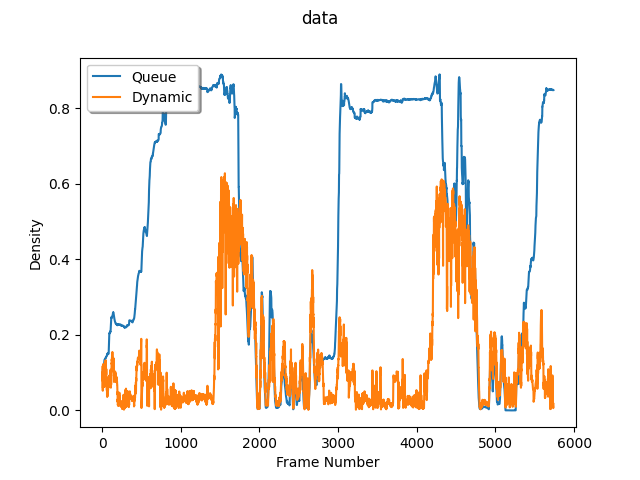
\includegraphics[width=15cm]{data.png}
    \caption{ Assignment 1 part (b)\\Total Runtime = 418 seconds}
    \label{fig:baseline}
\end{figure}

\subsection{Method - 1}
Figure 3.2 shows a typical output of Method - 1 wherein we have set x = 10 ( i.e, after processing Nth frame, we process N + 10th frame).

\begin{figure}[ht!]
    \centering
    \captionsetup{justification=centering,margin=2cm}
    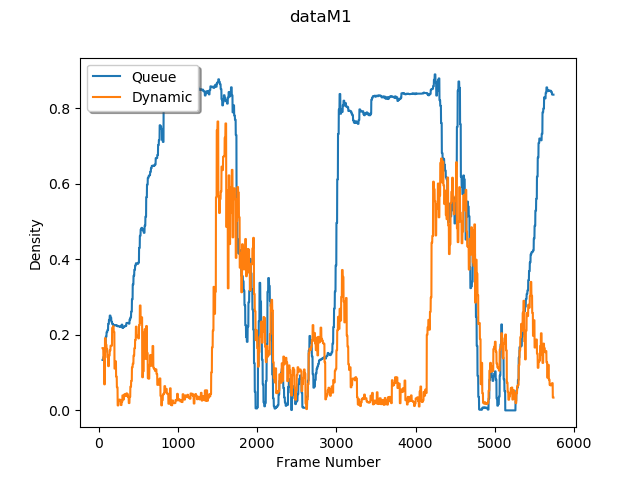
\includegraphics[width=15cm]{dataM1.png}
    \caption{ Method - 1: x = 10 \\Total Runtime = 63 seconds}
    \label{fig:typicalM1}
\end{figure}




\begin{comment}
\subsection{Heading on level 2 (subsection)}
Lorem ipsum 
\begin{align}
	A = 
	\begin{bmatrix}
	A_{11} & A_{21} \\
  	A_{21} & A_{22}
	\end{bmatrix}
\end{align}
Aenean commodo

\subsubsection{Heading on level 3 (subsubsection)}
Nulla consequat 

\paragraph{Heading on level 4 (paragraph)}
Lorem ipsum 

\section{Lists}

\subsection{Example for list (3*itemize)}
\begin{itemize}
	\item First item in a list 
		\begin{itemize}
		\item First item in a list 
			\begin{itemize}
			\item First item in a list 
			\item Second item in a list 
			\end{itemize}
		\item Second item in a list 
		\end{itemize}
	\item Second item in a list 
\end{itemize}

\subsection{Example for list (enumerate)}
\begin{enumerate}
	\item First item in a list 
	\item Second item in a list 
	\item Third item in a list
\end{enumerate}
\end{comment}

























%%% End document
\end{document}
